\question Clasifica los cuerpos geométricos.
\begin{center}
    \dashedbox{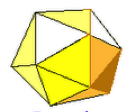
\includegraphics[width=0.18\textwidth ]{../images/sinma2_aiu3_ac79_img01}} \qquad
    \dashedbox{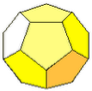
\includegraphics[width=0.18\textwidth ]{../images/sinma2_aiu3_ac79_img02}} \qquad
    \dashedbox{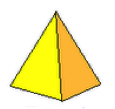
\includegraphics[width=0.18\textwidth ]{../images/sinma2_aiu3_ac79_img03}} \qquad
    \dashedbox{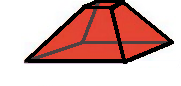
\includegraphics[width=0.18\textwidth ]{../images/sinma2_aiu3_ac79_img04}} \qquad
    \dashedbox{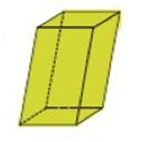
\includegraphics[width=0.18\textwidth ]{../images/sinma2_aiu3_ac79_img05}} \qquad
    \dashedbox{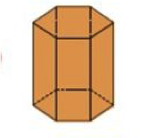
\includegraphics[width=0.18\textwidth ]{../images/sinma2_aiu3_ac79_img06}} \qquad
    \dashedbox{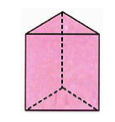
\includegraphics[width=0.18\textwidth ]{../images/sinma2_aiu3_ac79_img07}} \qquad
\end{center}

\begin{multicols}{2}
    \fbox{
        \begin{minipage}[t]{0.8\linewidth}
            Prisma recto \vspace{6cm}
        \end{minipage}
    }
    \fbox{
        \begin{minipage}[t]{0.8\linewidth}
            Otro \vspace{6cm}
        \end{minipage}
    }
\end{multicols}
